\section{Experiments}



\subsection{Datasets}

\subsection{Single Model Visualization on ImageNet}

\subsection{Class Model Visualization on Multiple Object Images}

\subsection{Construction Visualization}

\subsection{Localization}

\begin{table}
\centering
Evaluation on Imagenet 2014 localization test set
\begin{tabular}{|c|c|c|}
\hline
Method & Localization error & Classification error\\
\hline
VggNet-Supervised[] & 25.3 & 7.4 \\
GoogleNet-Supervised [] & 26.4 & 14.8 \\
AlexNet-Weakly[] & & \\
AlexNet-Weakly Feedback & & \\
VggNet-Weakly Feedback & & \\
GooglNet-Weakl Feedback & & \\
\hline
\end{tabular}
\caption{We show the localization evaluation on ImageNet 2014 localization competition. Our model clearly outperforms the weakly supervised approach based on []. Notably, we compare even fairbly well against supervisedly trained localization model, where an extra localization bouding boxes dataset is used. We demonstrate that when learning for classifications objectives, the Deep ConvNet already integrate powerful class specific features for attentioning on the important areas.}
\label{tab:localization_accuracy}
\end{table}

\setlength{\tabcolsep}{2pt}
\begin{figure*}
\begin{center}
\begin{tabular}{cc}
%\rotatebox{90}{\hspace{5mm}Sequential} &
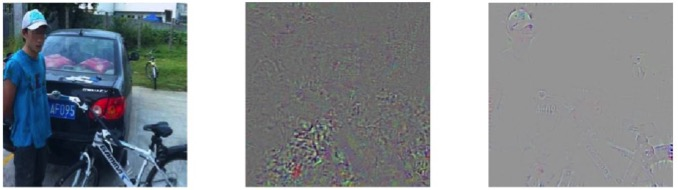
\includegraphics[width=0.45\linewidth]{figs/examples/bic-car1_bike} &
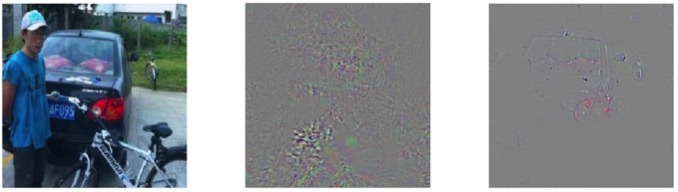
\includegraphics[width=0.45\linewidth]{figs/examples/bic-car1_car} \\
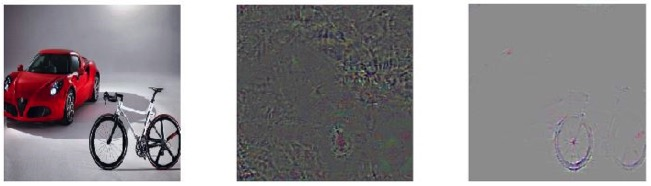
\includegraphics[width=0.45\linewidth]{figs/examples/bic-car2_bike} &
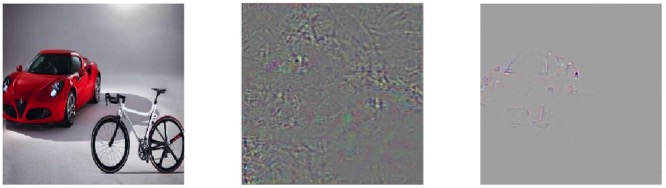
\includegraphics[width=0.45\linewidth]{figs/examples/bic-car2_car} \\
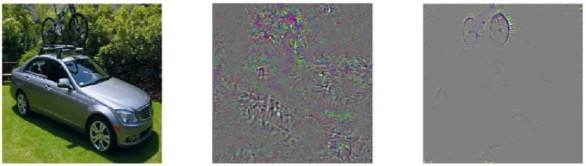
\includegraphics[width=0.45\linewidth]{figs/examples/bic-car3_bike} &
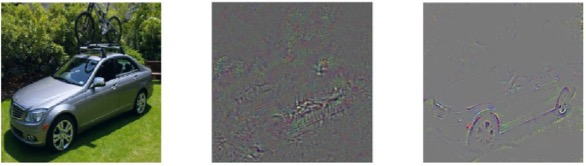
\includegraphics[width=0.45\linewidth]{figs/examples/bic-car3_car} \\ 
{\small (a) Bike} &
{\small (b) Car} \\
\end{tabular}
% \vspace{-10pt}
\caption{We show more qualitative results of our feedback neural network on natual images. For each image, we show the original image gradient w.r.t. the class labels and the updated image gradients w.r.t. class labels after feedback. We select a few images for comparing bike v.s. car, zebra v.s. elephant, dog v.s. cat, indicating that our approach can find the targeted objects given only a trained feedforward convnets and class labels.} 
\label{fig:examples}
% \vspace{-30pt}
\end{center}
\end{figure*}
